% SDCNN Architecture — TikZ diagram
% Include in main.tex with:  % SDCNN Architecture — TikZ diagram
% Include in main.tex with:  % SDCNN Architecture — TikZ diagram
% Include in main.tex with:  % SDCNN Architecture — TikZ diagram
% Include in main.tex with:  \input{figures/sdcnn_tikz}
% Or compile standalone:     pdflatex sdcnn_tikz.tex

\documentclass[border=5pt]{standalone}
\usepackage{tikz}
\usepackage{amsmath}
\usetikzlibrary{shapes.geometric, arrows.meta, positioning, fit, backgrounds, calc}

\begin{document}

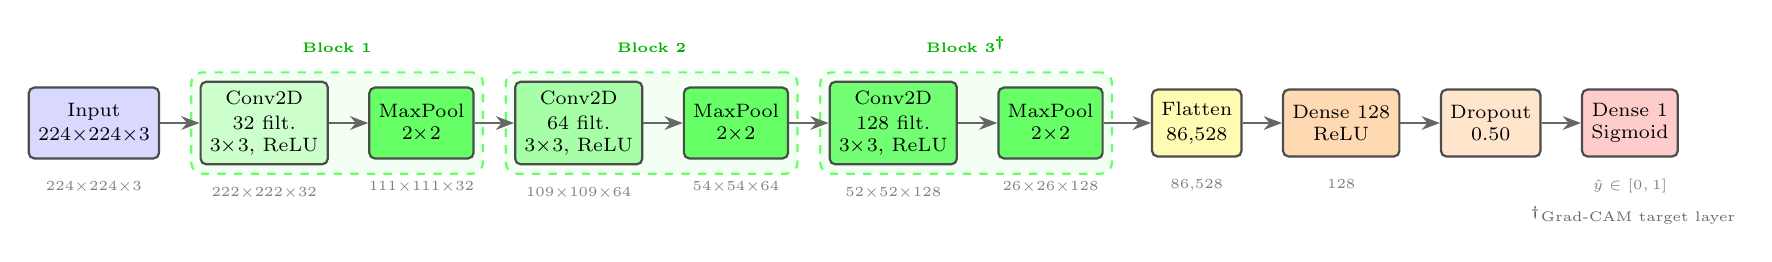
\begin{tikzpicture}[
  node distance = 0.35cm and 0.5cm,
  block/.style = {rectangle, draw=black!70, thick, fill=#1,
                  minimum width=1.2cm, minimum height=0.9cm,
                  font=\scriptsize, align=center, rounded corners=2pt},
  pool/.style  = {rectangle, draw=black!70, thick, fill=#1!60,
                  minimum width=0.7cm, minimum height=0.9cm,
                  font=\scriptsize, align=center, rounded corners=2pt},
  head/.style  = {rectangle, draw=black!70, thick, fill=#1,
                  minimum width=1.0cm, minimum height=0.85cm,
                  font=\scriptsize, align=center, rounded corners=2pt},
  arr/.style   = {-Stealth, thick, draw=black!60},
  lbl/.style   = {font=\tiny, text=gray},
]

% ── Input ─────────────────────────────────────────────────────────────────────
\node[block=blue!15] (inp) {Input\\[1pt]$224{\times}224{\times}3$};

% ── Block 1 ────────────────────────────────────────────────────────────────────
\node[block=green!20, right=of inp] (c1)  {Conv2D\\[1pt]32 filt.\\3×3, ReLU};
\node[pool=green,     right=of c1]  (p1)  {MaxPool\\2×2};

% ── Block 2 ────────────────────────────────────────────────────────────────────
\node[block=green!35, right=of p1] (c2)  {Conv2D\\[1pt]64 filt.\\3×3, ReLU};
\node[pool=green,     right=of c2] (p2)  {MaxPool\\2×2};

% ── Block 3 ────────────────────────────────────────────────────────────────────
\node[block=green!55, right=of p2] (c3)  {Conv2D\\[1pt]128 filt.\\3×3, ReLU};
\node[pool=green,     right=of c3] (p3)  {MaxPool\\2×2};

% ── Flatten ────────────────────────────────────────────────────────────────────
\node[head=yellow!30, right=0.6cm of p3] (flat) {Flatten\\[1pt]86{,}528};

% ── Dense + Dropout ────────────────────────────────────────────────────────────
\node[head=orange!30, right=of flat] (d1)  {Dense 128\\ReLU};
\node[head=orange!20, right=of d1]   (do)  {Dropout\\0.50};

% ── Output ─────────────────────────────────────────────────────────────────────
\node[head=red!20, right=of do] (out) {Dense 1\\Sigmoid};

% ── Arrows ─────────────────────────────────────────────────────────────────────
\foreach \from/\to in {inp/c1, c1/p1, p1/c2, c2/p2, p2/c3, c3/p3,
                        p3/flat, flat/d1, d1/do, do/out}
  \draw[arr] (\from) -- (\to);

% ── Feature-map size labels ──────────────────────────────────────────────────
\node[lbl, below=0.15cm of inp] {$224{\times}224{\times}3$};
\node[lbl, below=0.15cm of c1]  {$222{\times}222{\times}32$};
\node[lbl, below=0.15cm of p1]  {$111{\times}111{\times}32$};
\node[lbl, below=0.15cm of c2]  {$109{\times}109{\times}64$};
\node[lbl, below=0.15cm of p2]  {$54{\times}54{\times}64$};
\node[lbl, below=0.15cm of c3]  {$52{\times}52{\times}128$};
\node[lbl, below=0.15cm of p3]  {$26{\times}26{\times}128$};
\node[lbl, below=0.15cm of flat]{86{,}528};
\node[lbl, below=0.15cm of d1] {128};
\node[lbl, below=0.15cm of out] {$\hat{y} \in [0,1]$};

% ── Block group labels ────────────────────────────────────────────────────────
\begin{scope}[on background layer]
  \node[draw=green!60, dashed, thick, rounded corners=4pt,
        fit=(c1)(p1), inner sep=3pt, fill=green!5] (b1box) {};
  \node[draw=green!60, dashed, thick, rounded corners=4pt,
        fit=(c2)(p2), inner sep=3pt, fill=green!5] (b2box) {};
  \node[draw=green!60, dashed, thick, rounded corners=4pt,
        fit=(c3)(p3), inner sep=3pt, fill=green!5] (b3box) {};
\end{scope}

\node[lbl, above=0.12cm of b1box, text=green!70!black, font=\tiny\bfseries] {Block 1};
\node[lbl, above=0.12cm of b2box, text=green!70!black, font=\tiny\bfseries] {Block 2};
\node[lbl, above=0.12cm of b3box, text=green!70!black, font=\tiny\bfseries] {Block 3\textsuperscript{\dag}};

% ── Grad-CAM footnote ─────────────────────────────────────────────────────────
\node[lbl, below right=0.5cm and -2cm of out, text=black!60]
  {\textsuperscript{\dag}Grad-CAM target layer};

\end{tikzpicture}

\end{document}

% Or compile standalone:     pdflatex sdcnn_tikz.tex

\documentclass[border=5pt]{standalone}
\usepackage{tikz}
\usepackage{amsmath}
\usetikzlibrary{shapes.geometric, arrows.meta, positioning, fit, backgrounds, calc}

\begin{document}

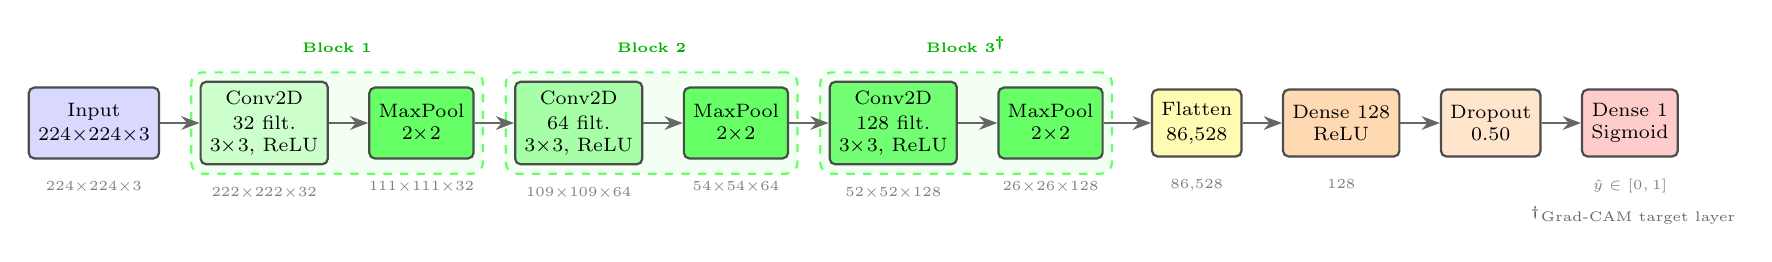
\begin{tikzpicture}[
  node distance = 0.35cm and 0.5cm,
  block/.style = {rectangle, draw=black!70, thick, fill=#1,
                  minimum width=1.2cm, minimum height=0.9cm,
                  font=\scriptsize, align=center, rounded corners=2pt},
  pool/.style  = {rectangle, draw=black!70, thick, fill=#1!60,
                  minimum width=0.7cm, minimum height=0.9cm,
                  font=\scriptsize, align=center, rounded corners=2pt},
  head/.style  = {rectangle, draw=black!70, thick, fill=#1,
                  minimum width=1.0cm, minimum height=0.85cm,
                  font=\scriptsize, align=center, rounded corners=2pt},
  arr/.style   = {-Stealth, thick, draw=black!60},
  lbl/.style   = {font=\tiny, text=gray},
]

% ── Input ─────────────────────────────────────────────────────────────────────
\node[block=blue!15] (inp) {Input\\[1pt]$224{\times}224{\times}3$};

% ── Block 1 ────────────────────────────────────────────────────────────────────
\node[block=green!20, right=of inp] (c1)  {Conv2D\\[1pt]32 filt.\\3×3, ReLU};
\node[pool=green,     right=of c1]  (p1)  {MaxPool\\2×2};

% ── Block 2 ────────────────────────────────────────────────────────────────────
\node[block=green!35, right=of p1] (c2)  {Conv2D\\[1pt]64 filt.\\3×3, ReLU};
\node[pool=green,     right=of c2] (p2)  {MaxPool\\2×2};

% ── Block 3 ────────────────────────────────────────────────────────────────────
\node[block=green!55, right=of p2] (c3)  {Conv2D\\[1pt]128 filt.\\3×3, ReLU};
\node[pool=green,     right=of c3] (p3)  {MaxPool\\2×2};

% ── Flatten ────────────────────────────────────────────────────────────────────
\node[head=yellow!30, right=0.6cm of p3] (flat) {Flatten\\[1pt]86{,}528};

% ── Dense + Dropout ────────────────────────────────────────────────────────────
\node[head=orange!30, right=of flat] (d1)  {Dense 128\\ReLU};
\node[head=orange!20, right=of d1]   (do)  {Dropout\\0.50};

% ── Output ─────────────────────────────────────────────────────────────────────
\node[head=red!20, right=of do] (out) {Dense 1\\Sigmoid};

% ── Arrows ─────────────────────────────────────────────────────────────────────
\foreach \from/\to in {inp/c1, c1/p1, p1/c2, c2/p2, p2/c3, c3/p3,
                        p3/flat, flat/d1, d1/do, do/out}
  \draw[arr] (\from) -- (\to);

% ── Feature-map size labels ──────────────────────────────────────────────────
\node[lbl, below=0.15cm of inp] {$224{\times}224{\times}3$};
\node[lbl, below=0.15cm of c1]  {$222{\times}222{\times}32$};
\node[lbl, below=0.15cm of p1]  {$111{\times}111{\times}32$};
\node[lbl, below=0.15cm of c2]  {$109{\times}109{\times}64$};
\node[lbl, below=0.15cm of p2]  {$54{\times}54{\times}64$};
\node[lbl, below=0.15cm of c3]  {$52{\times}52{\times}128$};
\node[lbl, below=0.15cm of p3]  {$26{\times}26{\times}128$};
\node[lbl, below=0.15cm of flat]{86{,}528};
\node[lbl, below=0.15cm of d1] {128};
\node[lbl, below=0.15cm of out] {$\hat{y} \in [0,1]$};

% ── Block group labels ────────────────────────────────────────────────────────
\begin{scope}[on background layer]
  \node[draw=green!60, dashed, thick, rounded corners=4pt,
        fit=(c1)(p1), inner sep=3pt, fill=green!5] (b1box) {};
  \node[draw=green!60, dashed, thick, rounded corners=4pt,
        fit=(c2)(p2), inner sep=3pt, fill=green!5] (b2box) {};
  \node[draw=green!60, dashed, thick, rounded corners=4pt,
        fit=(c3)(p3), inner sep=3pt, fill=green!5] (b3box) {};
\end{scope}

\node[lbl, above=0.12cm of b1box, text=green!70!black, font=\tiny\bfseries] {Block 1};
\node[lbl, above=0.12cm of b2box, text=green!70!black, font=\tiny\bfseries] {Block 2};
\node[lbl, above=0.12cm of b3box, text=green!70!black, font=\tiny\bfseries] {Block 3\textsuperscript{\dag}};

% ── Grad-CAM footnote ─────────────────────────────────────────────────────────
\node[lbl, below right=0.5cm and -2cm of out, text=black!60]
  {\textsuperscript{\dag}Grad-CAM target layer};

\end{tikzpicture}

\end{document}

% Or compile standalone:     pdflatex sdcnn_tikz.tex

\documentclass[border=5pt]{standalone}
\usepackage{tikz}
\usepackage{amsmath}
\usetikzlibrary{shapes.geometric, arrows.meta, positioning, fit, backgrounds, calc}

\begin{document}

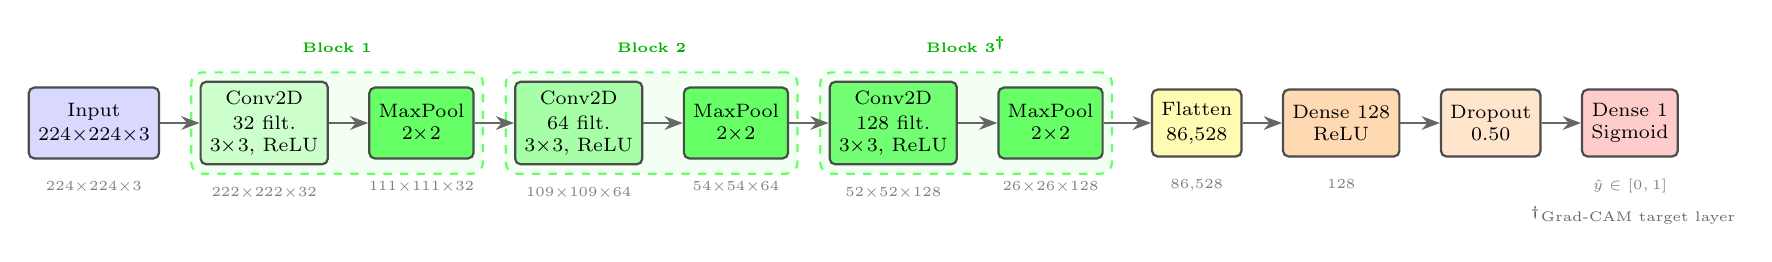
\begin{tikzpicture}[
  node distance = 0.35cm and 0.5cm,
  block/.style = {rectangle, draw=black!70, thick, fill=#1,
                  minimum width=1.2cm, minimum height=0.9cm,
                  font=\scriptsize, align=center, rounded corners=2pt},
  pool/.style  = {rectangle, draw=black!70, thick, fill=#1!60,
                  minimum width=0.7cm, minimum height=0.9cm,
                  font=\scriptsize, align=center, rounded corners=2pt},
  head/.style  = {rectangle, draw=black!70, thick, fill=#1,
                  minimum width=1.0cm, minimum height=0.85cm,
                  font=\scriptsize, align=center, rounded corners=2pt},
  arr/.style   = {-Stealth, thick, draw=black!60},
  lbl/.style   = {font=\tiny, text=gray},
]

% ── Input ─────────────────────────────────────────────────────────────────────
\node[block=blue!15] (inp) {Input\\[1pt]$224{\times}224{\times}3$};

% ── Block 1 ────────────────────────────────────────────────────────────────────
\node[block=green!20, right=of inp] (c1)  {Conv2D\\[1pt]32 filt.\\3×3, ReLU};
\node[pool=green,     right=of c1]  (p1)  {MaxPool\\2×2};

% ── Block 2 ────────────────────────────────────────────────────────────────────
\node[block=green!35, right=of p1] (c2)  {Conv2D\\[1pt]64 filt.\\3×3, ReLU};
\node[pool=green,     right=of c2] (p2)  {MaxPool\\2×2};

% ── Block 3 ────────────────────────────────────────────────────────────────────
\node[block=green!55, right=of p2] (c3)  {Conv2D\\[1pt]128 filt.\\3×3, ReLU};
\node[pool=green,     right=of c3] (p3)  {MaxPool\\2×2};

% ── Flatten ────────────────────────────────────────────────────────────────────
\node[head=yellow!30, right=0.6cm of p3] (flat) {Flatten\\[1pt]86{,}528};

% ── Dense + Dropout ────────────────────────────────────────────────────────────
\node[head=orange!30, right=of flat] (d1)  {Dense 128\\ReLU};
\node[head=orange!20, right=of d1]   (do)  {Dropout\\0.50};

% ── Output ─────────────────────────────────────────────────────────────────────
\node[head=red!20, right=of do] (out) {Dense 1\\Sigmoid};

% ── Arrows ─────────────────────────────────────────────────────────────────────
\foreach \from/\to in {inp/c1, c1/p1, p1/c2, c2/p2, p2/c3, c3/p3,
                        p3/flat, flat/d1, d1/do, do/out}
  \draw[arr] (\from) -- (\to);

% ── Feature-map size labels ──────────────────────────────────────────────────
\node[lbl, below=0.15cm of inp] {$224{\times}224{\times}3$};
\node[lbl, below=0.15cm of c1]  {$222{\times}222{\times}32$};
\node[lbl, below=0.15cm of p1]  {$111{\times}111{\times}32$};
\node[lbl, below=0.15cm of c2]  {$109{\times}109{\times}64$};
\node[lbl, below=0.15cm of p2]  {$54{\times}54{\times}64$};
\node[lbl, below=0.15cm of c3]  {$52{\times}52{\times}128$};
\node[lbl, below=0.15cm of p3]  {$26{\times}26{\times}128$};
\node[lbl, below=0.15cm of flat]{86{,}528};
\node[lbl, below=0.15cm of d1] {128};
\node[lbl, below=0.15cm of out] {$\hat{y} \in [0,1]$};

% ── Block group labels ────────────────────────────────────────────────────────
\begin{scope}[on background layer]
  \node[draw=green!60, dashed, thick, rounded corners=4pt,
        fit=(c1)(p1), inner sep=3pt, fill=green!5] (b1box) {};
  \node[draw=green!60, dashed, thick, rounded corners=4pt,
        fit=(c2)(p2), inner sep=3pt, fill=green!5] (b2box) {};
  \node[draw=green!60, dashed, thick, rounded corners=4pt,
        fit=(c3)(p3), inner sep=3pt, fill=green!5] (b3box) {};
\end{scope}

\node[lbl, above=0.12cm of b1box, text=green!70!black, font=\tiny\bfseries] {Block 1};
\node[lbl, above=0.12cm of b2box, text=green!70!black, font=\tiny\bfseries] {Block 2};
\node[lbl, above=0.12cm of b3box, text=green!70!black, font=\tiny\bfseries] {Block 3\textsuperscript{\dag}};

% ── Grad-CAM footnote ─────────────────────────────────────────────────────────
\node[lbl, below right=0.5cm and -2cm of out, text=black!60]
  {\textsuperscript{\dag}Grad-CAM target layer};

\end{tikzpicture}

\end{document}

% Or compile standalone:     pdflatex sdcnn_tikz.tex

\documentclass[border=5pt]{standalone}
\usepackage{tikz}
\usepackage{amsmath}
\usetikzlibrary{shapes.geometric, arrows.meta, positioning, fit, backgrounds, calc}

\begin{document}

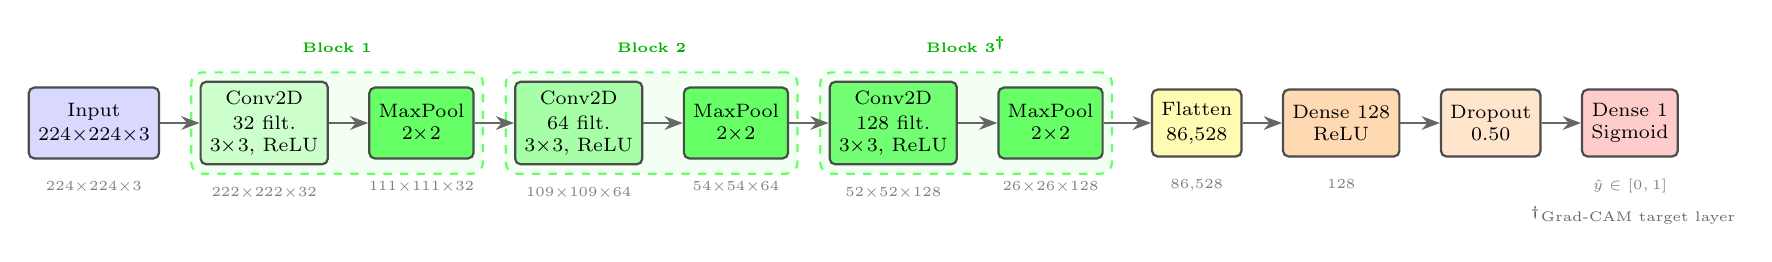
\begin{tikzpicture}[
  node distance = 0.35cm and 0.5cm,
  block/.style = {rectangle, draw=black!70, thick, fill=#1,
                  minimum width=1.2cm, minimum height=0.9cm,
                  font=\scriptsize, align=center, rounded corners=2pt},
  pool/.style  = {rectangle, draw=black!70, thick, fill=#1!60,
                  minimum width=0.7cm, minimum height=0.9cm,
                  font=\scriptsize, align=center, rounded corners=2pt},
  head/.style  = {rectangle, draw=black!70, thick, fill=#1,
                  minimum width=1.0cm, minimum height=0.85cm,
                  font=\scriptsize, align=center, rounded corners=2pt},
  arr/.style   = {-Stealth, thick, draw=black!60},
  lbl/.style   = {font=\tiny, text=gray},
]

% ── Input ─────────────────────────────────────────────────────────────────────
\node[block=blue!15] (inp) {Input\\[1pt]$224{\times}224{\times}3$};

% ── Block 1 ────────────────────────────────────────────────────────────────────
\node[block=green!20, right=of inp] (c1)  {Conv2D\\[1pt]32 filt.\\3×3, ReLU};
\node[pool=green,     right=of c1]  (p1)  {MaxPool\\2×2};

% ── Block 2 ────────────────────────────────────────────────────────────────────
\node[block=green!35, right=of p1] (c2)  {Conv2D\\[1pt]64 filt.\\3×3, ReLU};
\node[pool=green,     right=of c2] (p2)  {MaxPool\\2×2};

% ── Block 3 ────────────────────────────────────────────────────────────────────
\node[block=green!55, right=of p2] (c3)  {Conv2D\\[1pt]128 filt.\\3×3, ReLU};
\node[pool=green,     right=of c3] (p3)  {MaxPool\\2×2};

% ── Flatten ────────────────────────────────────────────────────────────────────
\node[head=yellow!30, right=0.6cm of p3] (flat) {Flatten\\[1pt]86{,}528};

% ── Dense + Dropout ────────────────────────────────────────────────────────────
\node[head=orange!30, right=of flat] (d1)  {Dense 128\\ReLU};
\node[head=orange!20, right=of d1]   (do)  {Dropout\\0.50};

% ── Output ─────────────────────────────────────────────────────────────────────
\node[head=red!20, right=of do] (out) {Dense 1\\Sigmoid};

% ── Arrows ─────────────────────────────────────────────────────────────────────
\foreach \from/\to in {inp/c1, c1/p1, p1/c2, c2/p2, p2/c3, c3/p3,
                        p3/flat, flat/d1, d1/do, do/out}
  \draw[arr] (\from) -- (\to);

% ── Feature-map size labels ──────────────────────────────────────────────────
\node[lbl, below=0.15cm of inp] {$224{\times}224{\times}3$};
\node[lbl, below=0.15cm of c1]  {$222{\times}222{\times}32$};
\node[lbl, below=0.15cm of p1]  {$111{\times}111{\times}32$};
\node[lbl, below=0.15cm of c2]  {$109{\times}109{\times}64$};
\node[lbl, below=0.15cm of p2]  {$54{\times}54{\times}64$};
\node[lbl, below=0.15cm of c3]  {$52{\times}52{\times}128$};
\node[lbl, below=0.15cm of p3]  {$26{\times}26{\times}128$};
\node[lbl, below=0.15cm of flat]{86{,}528};
\node[lbl, below=0.15cm of d1] {128};
\node[lbl, below=0.15cm of out] {$\hat{y} \in [0,1]$};

% ── Block group labels ────────────────────────────────────────────────────────
\begin{scope}[on background layer]
  \node[draw=green!60, dashed, thick, rounded corners=4pt,
        fit=(c1)(p1), inner sep=3pt, fill=green!5] (b1box) {};
  \node[draw=green!60, dashed, thick, rounded corners=4pt,
        fit=(c2)(p2), inner sep=3pt, fill=green!5] (b2box) {};
  \node[draw=green!60, dashed, thick, rounded corners=4pt,
        fit=(c3)(p3), inner sep=3pt, fill=green!5] (b3box) {};
\end{scope}

\node[lbl, above=0.12cm of b1box, text=green!70!black, font=\tiny\bfseries] {Block 1};
\node[lbl, above=0.12cm of b2box, text=green!70!black, font=\tiny\bfseries] {Block 2};
\node[lbl, above=0.12cm of b3box, text=green!70!black, font=\tiny\bfseries] {Block 3\textsuperscript{\dag}};

% ── Grad-CAM footnote ─────────────────────────────────────────────────────────
\node[lbl, below right=0.5cm and -2cm of out, text=black!60]
  {\textsuperscript{\dag}Grad-CAM target layer};

\end{tikzpicture}

\end{document}
